% \documentclass[12pt]{book}
% \usepackage[spanish]{babel}
% \usepackage[utf8x]{inputenc}
% \usepackage[T1]{fontenc}
% \usepackage[utf8]{inputenc}
% \usepackage{amsfonts}
% \usepackage{fancyhdr}
% \usepackage{MnSymbol}
% \usepackage{graphicx}
% \usepackage{float}
% \usepackage{wasysym}
% %\usepackage[spanish]{babel}
% \usepackage{pdfpages}
% \usepackage[margin=0.5in,left=1in,right=1.5in, bottom = 1.5in, includehead]{geometry}
% \usepackage{amsmath}
% \usepackage{multicol}
% \renewcommand{\baselinestretch}{1.5}  

\documentclass[12pt]{article}
\usepackage[T1]{fontenc}
\usepackage[utf8]{inputenc}
\usepackage[spanish]{babel}
\usepackage{amsmath}
\usepackage{MnSymbol}
\usepackage{wasysym}
\usepackage{multicol}
\setlength{\columnsep}{1cm}
\usepackage[margin=2.5cm,left=3cm, includehead]{geometry}
\usepackage{graphicx}
\usepackage{float}
\usepackage{fancyhdr}
\usepackage{cancel}
\usepackage{pgf,tikz}
\usepackage{mathrsfs}
\usetikzlibrary{arrows}
\usepackage{amsthm}
\usepackage{amsfonts}
\renewcommand{\baselinestretch}{1.2}
\usepackage{cite}




%% NEW Comands
\newcommand{\R}{\mathbb R}  
\newcommand{\N}{\mathbb N}  
\newcommand{\Z}{\mathbb Z}  


\title{Reporte Enero 2021}
\author{Jorge Ballote}
\begin{document}
\maketitle
\section{Introducción}
Éste no es un reporte formal, sólo un pequeño informe de mis avances. Presento mis dudas.
\section{Teoría}
En el artículo \cite{surveyODEforDL} aparece el siguiente texto:
\begin{figure}[H]
    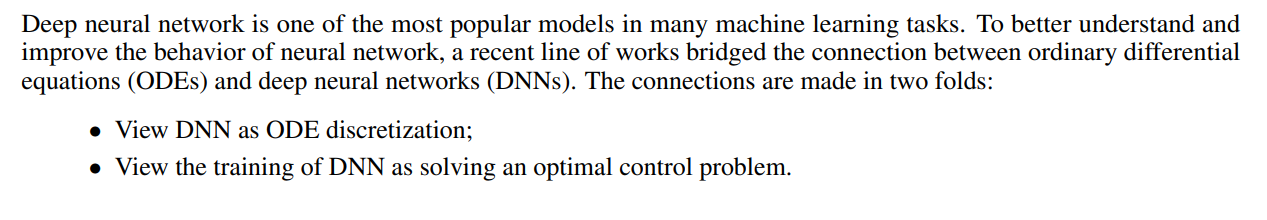
\includegraphics[height=1.1in]{../src/duda1.png}
\end{figure}
Pero yo he sentido que he leído de ambos temas. La idea de contruír una red basada en Runge Kutta simpléctico sería ver una DNN como una discretización de ODE.

Por otro lado, también hemos estudiado el aprendizajede las redes como problema de control óptimo. 
¿Implica que algo interpretamos mal? ¿o que los resultados que buscamos son muy flexibles y podríamos indagar en ambos nichos?

\subsection{Runge Kutta simpléctico ¿Posible pero tardado?}
Los métodos simplécticos de Runge Kutta son esquemas implícitos para resolver ODEs. Antes de intentar hacer un Runge Kutta implícito, intenté ver como se resolvía Euler implícito:
\begin{equation}
    \label{1}
    x_{n+1} = x_n + h f(x_{n+1})
\end{equation}
Un ejemplo, podría ser la ecuación $\dot x = -kx$.
\begin{align*}
    x_{n+1} &= x_n + h (-kx_{n+1}) \\
        &=x_n -hkx_{n+1} \\ 
\end{align*}
Con lo que es posible despejar $x_{n+1}$
$$ x_{n+1} +hkx_{n+1} = x_n $$
$$ \Rightarrow x_{n+1}  = \frac{x_n}{1+hk}.$$
Sin embargo, ésta manera depende mucho de que sea posible despejar $x_{n+1}$ en términos de $x_n$. Al principio pensé que ésto haría imposible la tarea pero luego recapacité. La ecuación (\ref{1}) podemos verla como un problema de punto fijo, tomando $x = x_{n+1}$ y la constante $a=x_n$.
\begin{equation}
    hf(x) + a = x
\end{equation}
Sea $g = hg +a$, obtenemos la ecuación:
$$g(x) = x$$
Lo cuál se puede resolver con métodos de punto fijo tradicionales.

\section{Experimentación}
En cuánto a la copia de ResNet que tengo en el Colab. No fue muy difícil conseguir salvar y cargar el modelo.

Decidí correr unas 10 épocas para observar que tan bien se comportaba. Al cargar el modelo, la evaluación mostró un $100\%$ de accuracy para mi sorpresa. Al principio creí que el test Set pudo haber estado contenido en el training set y que eran imágenes que la red ya había visto. Pero revisando el código parece que no fue así. Sigo sospechando que algo no está bien. Entre mis planes está programar una matriz de confusión. 

\section{Redacción}
Empecé a redactar, no llevo demasiado. Pero me senté a definir un poco lo que habíamos estudiado y lo que me gustaría incluír. Comencé el capítulo de convoluciones y anexo con éste reporte lo que llevo escrito.
\bibliographystyle{unsrt}
\bibliography{papers}
    
\end{document}